\documentclass[12pt]{article}
\usepackage[a4paper, margin=.30in]{geometry}
\usepackage{graphicx ,
            wrapfig,
            xcolor, 
            enumerate,
            amsmath,fontenc,
            tcolorbox,mathrsfs
            }
\usepackage{mathptmx}
\usepackage[siunitx, RPvoltages]{circuitikz}
\newcommand\headerMe[2]{\noindent{}#1\hfill#2}
\renewcommand{\thesection}{\Roman{section}}

\author{Zakaria HAOUZAN}
\date{\today}

\begin{document}
% headers --------------
\headerMe{Matière : Physique-Chimie}{Professeur : Zakaria HAOUZAN}\\
\headerMe{Unité : Electricité}{Établissement : Lycée SKHOR qualifiant}\\
\headerMe{Niveau : 1BAC-SM/X}{Heure : 17H/12H}\\

% ------Content ________

%\begin{wrapfigure}[10]{r}{0.5\textwidth}
    %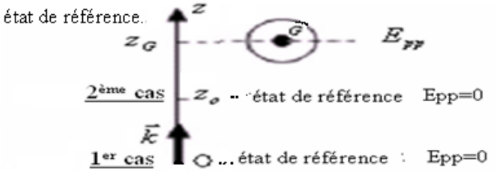
\includegraphics[width=0.5\textwidth]{./img/img00.png}
%\end{wrapfigure}


%\begin{tcolorbox}[colback=black!15!white,
                  %colframe=black!10!black,
                  %title=Remarque :
                 %]
\begin{center}

    \Large{Leçon $N^{\circ} 8 $: \color{red}Champ magnétique }
\end{center}

\begin{wrapfigure}[]{r}{0.2\textwidth}
  \vspace{-1cm}
    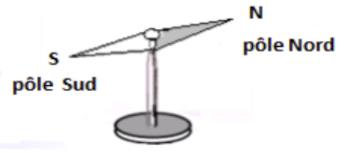
\includegraphics[width=0.2\textwidth]{./img/boussole.png}
\end{wrapfigure}
  \section{ champ magnétique créé par un aimant:}
  \subsection{L’aiguille aimanté :}
La boussole est une aiguille aimantée mobile pivotant autour d'un axe vertical, elle permet de déterminer
l’existence d’un champ magnétique et de préciser son sens et sa direction.

Par convention, on appelle pôle nord de l’aiguille aimantée son pôle qui se dirige spontanément vers le nord et le

  pôle sud celui qui se dirige spontanément vers le sud .
Sous l’effet du champ magnétique terrestre le pôle nord de l’aiguille aimantée se dirige vers le nord.

\begin{wrapfigure}[]{r}{0.2\textwidth}
  \vspace{-2cm}
    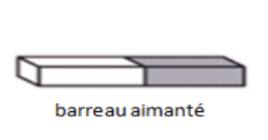
\includegraphics[width=0.2\textwidth]{./img/barreauAimante.png}
    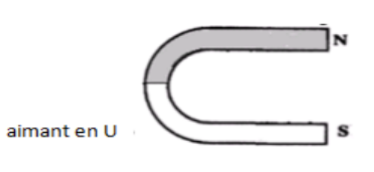
\includegraphics[width=0.2\textwidth]{./img/Aimant_U.png}
    
\end{wrapfigure}

 
  \subsection{L’ aimant :}
Un aimant est un corps capable d'attirer le fer, le nickel, le cobalt et certains alliages contenant le fer (comme
l'acier); ces corps sont appelés corps ferromagnétiques.
On distingue les aimants en U et les barreaux aimantés.

Chaque aimant possède un pôle nord et un pôle sud.
On fait l’expérience de l’aimant brisé qui montre que l’aimantation réapparaît et on a toujours un pôle sur le
bout coupé.

  On en déduit que le secret de l’aimantation réside dans le fait qu’un atome unique se comporte comme un aimant.

 \begin{wrapfigure}[7]{r}{0.2\textwidth}
  \vspace{-1cm}
    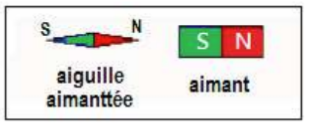
\includegraphics[width=0.2\textwidth]{./img/Action_aimant_boussole.png}

    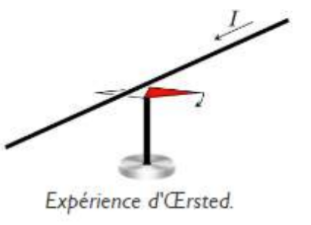
\includegraphics[width=0.2\textwidth]{./img/courant_boussole.png}
\end{wrapfigure}
 
   \section{Mise en évidence du champ magnétique :}
  \subsection{Action d’un aimant sur une aiguille aimantée :}

  Lorsqu’on approche une aiguille aimantée d’un aimant, on
constate qu’elle prend une position stable, on dit qu’il y a
une interaction entre l’aimant et l’aiguille aimanté.
 
  \begin{wrapfigure}[10]{r}{0.3\textwidth}
  \vspace{-3cm}
    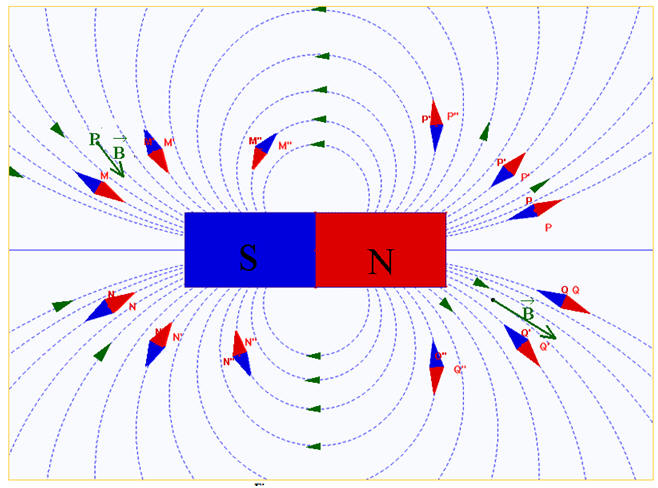
\includegraphics[width=0.3\textwidth]{./img/miseEnEvidence.jpg}
\end{wrapfigure}


  \subsection{Action d’un courant électrique sur une aiguille aimantée :}
  Une aiguille aimantée dévie au voisinage d’un conducteur
parcouru par un courant électrique continu. Sa déviation
dépend du sens du courant qui traverse le conducteur.
    \section{Champ magnétique et spectres magnétiques :}
  \subsection{Vecteur champ magnétique : }
Plaçons différentes aiguilles aimantées et posons près d’elles un aimant .On constate que les aiguilles prennent des
directions différentes de celles qu’elles avaient auparavant.

L’aimant provoque une modification des propriétés de l’espace qui l’entoure car il crée autour de lui un champ
magnétique. Tout point du champ magnétique est caractérisé un vecteur champ magnétique $\vec{B}$
\subsection{Les caractéristiques du vecteur champ magnétique :}
Les caractéristiques du vecteur champ magnétique $\vec{B}$ en un point M sont:
\\Origine : le point M
\\- Direction : celle prise par l’aiguille aimantée placée en M
\\- Sens : celui qui indique le pôle nord de l’aiguille aimantée (du sud vers le nord de
l’aiguille)
\\- Valeur : (mesurée par un tesla-mètre) exprimée en Tesla (T).
\subsection{Les spectres magnétiques :}
\subsubsection{les lignes du champ :}
Une ligne de champ est une courbe qui est tangente aux vecteurs champs
magnétiques en chacun de ces points.
Le spectre magnétique est l’ensemble des lignes de champ.
Les lignes de champ sont orientées dans le sens du vecteur champ magnétique.
\begin{center}
    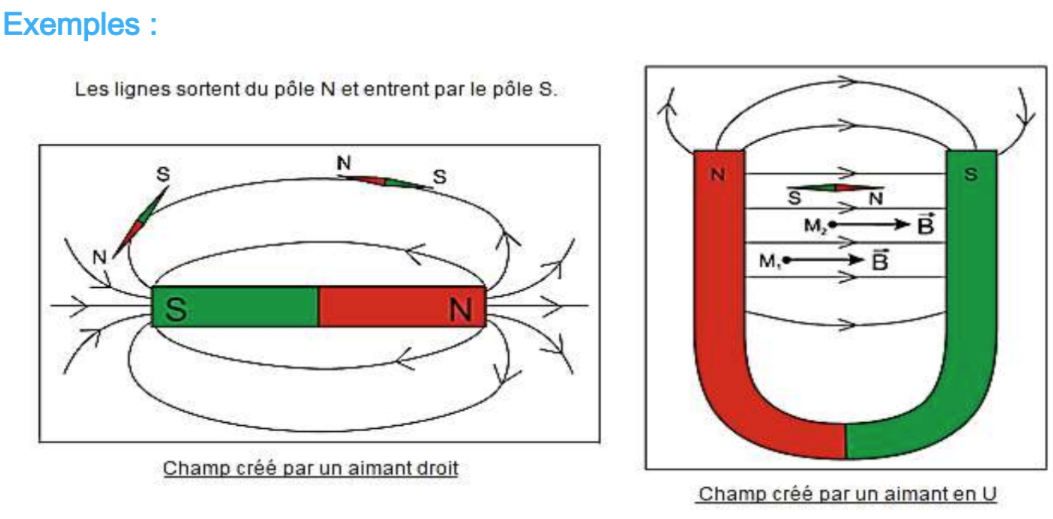
\includegraphics[width=0.7\textwidth]{./img/spectreMag_B.png}
\end{center}
\subsubsection{Champ magnétique uniforme :}
Un champ magnétique est uniforme dans une région de l’espace, si le vecteur champ
magnétique a les mêmes caractéristiques (directions, sens et valeur) en tout point de
cette région.
  
  \begin{wrapfigure}[10]{r}{0.4\textwidth}
    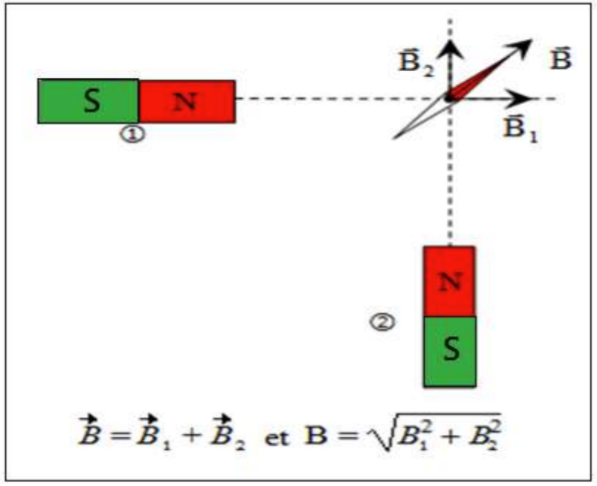
\includegraphics[width=0.4\textwidth]{./img/superpositio_mag_B.png}
\end{wrapfigure}

Le spectre du champ magnétique uniforme est formé de segments de droites
parallèles entres eux. C’est le cas dans l’entrefer d’un aimant en U.
\section{superposition de champs magnétiques :}
S’il y a plusieurs champs magnétiques (créés par plusieurs sources distinctes), le
vecteur champ magnétique résultant en un point est égal à la somme vectorielle des
champs créés par chacune des sources en ce point.
$$\vec{B} = \sum \vec{B}$$
  \section{Champ magnétique terrestre :}
Au tour de la terre règne un champ magnétique appelé champ géomagnétique.

Le pôle magnétique sud se trouve à proximité du pôle géographique nord. De même le
pôle magnétique nord se trouve près du pôle sud géographique.
\begin{center}

    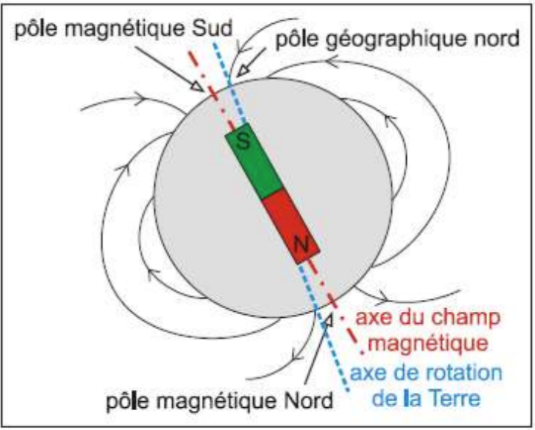
\includegraphics[width=0.5\textwidth]{./img/champ_terrestre.png}
\end{center}
Le camp magnétique terrestre (ou champ géomagnétique) ressemble à celui produit
par un aimant droit.
\\-Les boussoles s’orientent le long des lignes de champ magnétique terrestre.
\\- Le pôle nord de l’aiguille aimantée est attiré par le pole terrestre magnétique sud.
\\-Le champ magnétique terrestre n’est pas horizontal mais forme un angle avec
l’horizontale appelé inclinaison Î .
\\-On appelle le plan vertical dont se trouve l’aiguille : le plan méridien magnétique. 
\\On écrit : $$\vec{B_T} = \vec{B_H} + \vec{B_V}$$
$$B_T = \frac{B_H}{cos(\alpha)}$$
$\vec{B_H}$ : Composante horizontale du champ magnétique terrestre

$\vec{B_V}$ : Composante verticale du champ magnétique terrestre

    \includegraphics[width=0.6\textwidth]{./img/plan méridien.png}

\end{document}

